\documentclass[a4paper, 11pt, ngerman, fleqn]{article}
\usepackage[ansinew]{inputenc}
\usepackage{babel,ngerman}
\usepackage{ngerman}
\usepackage{coordsys,logsys,color}
\usepackage{texdraw}
\usepackage{fancyhdr}
\usepackage{rotating}
\usepackage{graphicx}

\pagestyle{fancy}

%\renewcommand{\familydefault}{cmss}

\definecolor{fgcgray}{rgb}{0.4, 0.4, 0.4}
\definecolor{warning}{rgb}{0.9, 0.1, 0.0}
\definecolor{bgctitle}{rgb}{0.5, 0.5, 0.5}
\definecolor{fgctitle}{rgb}{0.95, 0.95, 0.95}
\newcommand{\titlefont}[1]{\textcolor{fgctitle}{\fontfamily{cmss}\fontseries{bx}\fontshape{n}\fontsize{20.48}{0pt} \selectfont #1}}
\newcommand{\inversetitlefont}[1]{\textcolor{bgctitle}{\fontfamily{cmss}\fontseries{bx}\fontshape{n}\fontsize{20.48}{0pt} \selectfont #1}}

\addtolength{\oddsidemargin}{-1.0cm}
\addtolength{\evensidemargin}{-1.0cm}
\addtolength{\headwidth}{2.0cm}
\addtolength{\textwidth}{2.0cm}

\setlength{\parindent}{0cm}

\renewcommand{\labelitemi}{$\circ$}
\renewcommand{\labelitemii}{$\diamond$}

\newcommand{\spaceline}[1][8pt]{\vskip #1}
\newcommand{\comment}[1]{\spaceline[5pt] \textcolor{fgcgray}{\scriptsize #1} \spaceline[15pt]}
\newcommand{\attrname}[1]{\textcolor{fgcgray}{\scriptsize #1}}


\makeatletter

\newcommand*{\project}[1]{\gdef\@project{#1}}
\newcommand*{\version}[1]{\gdef\@version{#1}}
\newcommand*{\home}[1]{\gdef\@home{#1}}
\newcommand*{\homeref}[1]{\gdef\@homeref{#1}}
\newcommand*{\prerequisite}[1]{\gdef\@prerequisite{#1}}
\newcommand*{\prerequisiteref}[1]{\gdef\@prerequisiteref{#1}}

\def\@maketitle{
  %\begin{titlepage}
  \begin{center}
    \colorbox{bgctitle}{
      \parbox{\textwidth}{
        \spaceline
        \centering{\titlefont{\@title}}
        \par
        \spaceline
      }
    }
    \colorbox{white}{
      \parbox{\textwidth}{
        \spaceline
        \centering{\inversetitlefont{\@project}}
        \par
        \spaceline
      }
    }
  \end{center}
  \spaceline[1.5em] {
    \begin{flushright}
    \begin{tabular}[t]{rl}
      \attrname{Projekt:} & \@project ~ \@version \\
      \attrname{Voraussetzung:} & \href{\@prerequisiteref}{\@prerequisite} \\
      \attrname{Autor:} & \@author \\
      \attrname{Home:} & \href{\@homeref}{\@home} \\
      \attrname{letzte "Anderung:} & \@date
    \end{tabular}
    \end{flushright}
    \par
  }
  \spaceline[5.5em]
  %\end{titlepage}
}

\setcounter{secnumdepth}{4}
\setcounter{tocdepth}{4}
	 
\newcounter{subsubsubsection}[subsubsection]
\def\subsubsubsectionmark#1{}
\def\thesubsubsubsection{\thesubsubsection .\arabic{subsubsubsection}}
\def\subsubsubsection{\@startsection{subsubsubsection}{4}{\z@}{-3.25ex plus -1 ex minus -.2ex}{1.5ex plus .2ex}{\normalsize\bf}}
\def\l@subsubsubsection{\@dottedtocline{4}{4.8em}{4.2em}}

\makeatother

\everytexdraw{
  \drawdim cm \linewd 0.01
  \arrowheadtype t:T
  \arrowheadsize l:0.2 w:0.2
  \setgray 0.5
}

\newcommand{\xheight}{0.6}
\newcommand{\xlength}{0.6}
\newcommand{\yheighta}{1.0}
\newcommand{\yheightb}{0.8}
\newcommand{\yheightc}{0.6}
\newcommand{\yheightd}{0.5}
\newcommand{\yheighte}{0.4}
\newcommand{\yheightf}{0.35}

\newcommand{\xhline}{\rlvec({\xlength} 0)}
\newcommand{\xharrow}{\ravec(0.7 0)}
\newcommand{\xnext}{%\rlvec(0.05 0) \lpatt(0.04 0.04) \rlvec(0.15 0) \lpatt()
}

\newcommand{\xtext}[3][\xheight]{
  \bsegment
    \bsegment
      \setsegscale 0.5
      \textref h:L v:C  \htext({\xheight} -0.1){#3}
    \esegment
    \setsegscale 0.5 \lvec(0 #1)
    \setsegscale 1
    \rlvec(#2 0) \rlvec(0 -#1) \rlvec(-#2 0) \lvec(0 0)
    \savepos(#2 0)(*@x *@y)
  \esegment
  \move(*@x *@y)
}

\newcommand{\bxtext}[3][\xheight]{
  \setgray{0.1}
  \linewd{0.026}
  \xtext[\xheight]{#2}{#3}
  \linewd{0.01}
  \setgray{0.5}
}

\newcommand{\xstartpage}{\bxtext{2.1}{Startseite}}
\newcommand{\xmainpage}{\bxtext{2.3}{Hauptseite}}
\newcommand{\xusermenu}{\bxtext{2.9}{Benutzermenu}}
\newcommand{\xgamelist}{\bxtext{2.2}{Spieleliste}}
\newcommand{\xportfolio}{\bxtext{2.0}{Portfolio}}
\newcommand{\xaccount}{\xtext{3.8}{Kennung per \textsl{eMail}}}


\begin{document}
  \begin{titlepage}
    \begin{center}
        \vspace{1cm}
        
        \Huge
        \textbf{Pflichtenheft} \\		  \textbf{StarCar}
        
        \vspace{0.5cm}
        \LARGE
        Datenverarbeitung in der Technik
       
        \vspace{3cm}
        
        \textbf{Robert Graf}
        
        \vspace{1.7cm}
        
        \begin{figure}
			\centering
			
\includegraphics[width=0.7\linewidth]{OTHLogo.jpg}
			\label{pic:OTHLogo}
		\end{figure}

       
        \vfill
        
        Wintersemester 2017/18
        
        \vspace{0.8cm}
          \Large
        Technische Informatik\\
        Ostbayerische Technische Hochschule Regensburg\\
       \today
        
    \end{center}
\end{titlepage}
 \newpage
  \tableofcontents \newpage
  \section{Teamaufstellung}

Die Gruppe ist innerhalb des Faches \textit{Datenverarbeitung in der Technik} als Gruppe 2 bekannt.\\
\\
Gruppenmitglieder:
\begin{itemize}
\item Bauer Annkathrin
\item Billor Mehmet
\item Boemmel Florian
\item Graf Robert
\item Huber Simone
\item Scharnagl Dominik
\item Strobel Anja
\end{itemize}
 \newpage
  \section{Zielbestimmungen}


\textbf{StarCar} ist ein Projekt von Studenten der Ostbayrischen Technischen Hochschule Regensburg im Fach Datenverarbeitung in der Technik im Wintersemester 2017/18. 
Die Studierenden erarbeiten weitgehend selbst�ndig L�sungen f�r spezielle aktuelle Problemstellungen aus der Technischen Informatik und pr�sentieren diese. Die Teilnehmer lernen die speziellen Herausforderungen bei dem gleichzeitigen und verzahnten Entwurf von Hardware- und Softwareteilen eines Systems kennen. Erfahrung in effektiver Teamarbeit.\par
Um diese Ziele zu erreichen hat sich die Gruppe 2 auf einen Projektvorschlag der Projektbegleitung geeinigt. Das Projekt besteht aus einem mit Sensoren best�ckten Fahrzeugmodell, welches komplett Zusammengebaut, Verdrahtet und letztendlich Programmiert werden muss um von den Studenten erw�hlte aufgaben zu erf�llen.\par
Die Studenten einigten sich auf ein Leitprojekt, welches das Modellfahrzeug in einen steuerbaren Haushaltsroboter verwandelt.\par
Ziel des Prototyps ist es, ein multifunktionales teilautonomes Fahrzeug f�r den Heimgebrauch zu schaffen.
Das Projekt \textStarCar soll somit richtungsweisende Techniken vereinen und in heterogenen Szenarien einsetzen.


\subsection{Musskriterien}

\begin{itemize}
  \item Montage
    \begin{itemize}
		\item	Embedded-System aus prim�rem und sekund�ren Controller
		\item	physikalisch stabiler Aufbau des Gesamtprojektes
		\item	stabile Stromversorgung
		\item	korrekte Elektronik
		\item	maximale Bewegungsfreiheit und korrekte Anbringung motorisierter Komponenten
    \end{itemize}
  \item Konfiguration
	\begin{itemize}
		\item	korrekte Initialisierung der Controller-Software
		\item	funktionierende Kommunikation zwischen prim�ren und sekund�rem Controller
	\end{itemize}
  \item Sensorik
    \begin{itemize}
		\item	ein f�r sichere Fahrt und Raumerkennung ausreichendes Setup an funktionierenden und konfigurierten Sensoren
		\item	Verabeitung der Sensordaten zu einem standardisierten Datenformat
    \end{itemize}
  \item Fahrzeug
    \begin{itemize}
		\item	ansteuerbare Antriebsmotoren und Lenkung
		\item	vereinfachte Steuerungsschnittstelle
    \end{itemize}
  \item Raumerkennung
    \begin{itemize}
		\item	Kartenerstellung
		\item	kollisionsfreie Fahrt
		\item	Wegfindung
    \end{itemize}
  \item Steuerung
    \begin{itemize}
		\item	Steuerung �ber externes Medium
    \end{itemize}
  \item Dokumentation
    \begin{itemize}
		\item	Dokumentation des Arbeitsaufwandes
		\item	Dokumentation des Projektverlaufes
		\item	Dokumentation des Endprodukts
    \end{itemize}

%\item 
%    \begin{itemize}
%		\item
%    \end{itemize}

\end{itemize}

\subsection{Wunschkriterien}

\begin{itemize}
	\item	Steuerung durch XBox Controller
	\item	Steuerung durch Gesten
\end{itemize}

\subsection{Abgrenzungskriterien}

\begin{itemize}
  \item Das Projekt soll keine tats�chlichen Hausarbeiten ausf�hren, nur technische Eigenschaften eines solchen Produktes aufweisen.
\end{itemize}

\subsection{Gantt-Chart}

Das Gantt-Diagramm zeigt den erwarteten Projektverlauf, gibt Zeiteinsch�tzungen, Richtlinien und Deadlines an.

\begin{sidewaysfigure}

	\centering
	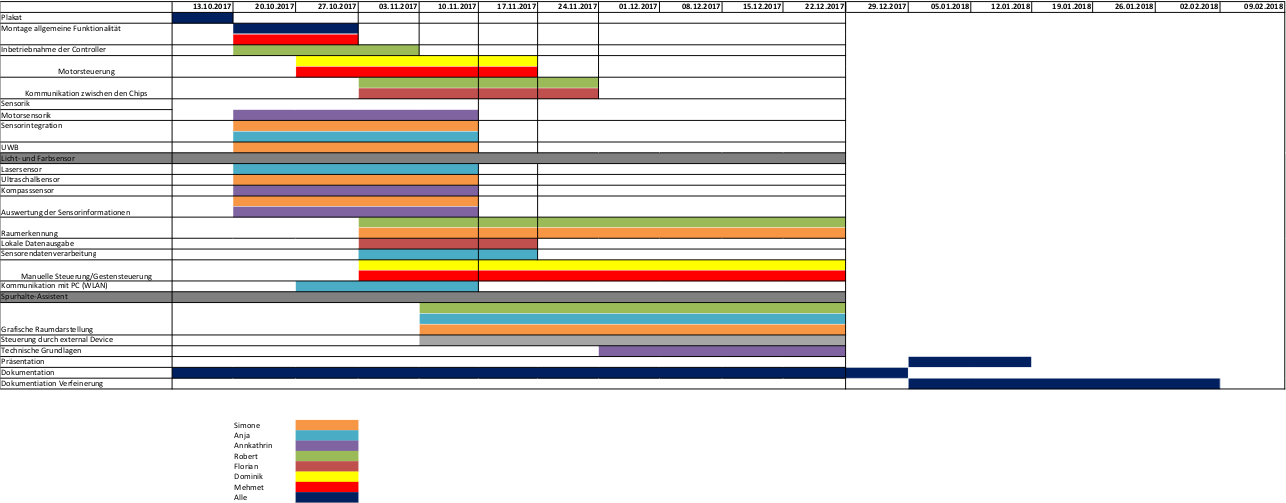
\includegraphics[width=200mm, height=130mm, scale=1]{Gantt_20_10.png}
	\caption{Gantt-Diagramm des erwarteten Projektverlaufs by Simone Huber}
	\label{fig:awesome_image}

\end{sidewaysfigure}

 \newpage
  \section{Produkteinsatz}

\comment{Welche Anwendungsbereiche (Zweck), Zielgruppen (Wer mit welchen Qualifikationen), Betriebsbedingungen (Betriebszeit, Aufsicht)?}

\subsection{Anwendungsbereiche}
Technologie f�r autonome Ger�tschaften hat viele Anwedungen. Vorstellbar sind automatische Staubsauger, Rasenm�her, Kellner, usw.
Ebenfalls denkbar ist der Einsatz in der Logistik als Kurzstreckentransportsystem.

\subsection{Zielgruppen}
Alle Personen, die ihren Alltag etwas mehr automatisieren wollen, k�nnen auf eine autonome Haushaltshilfe zur�ckgreifen. Die in diesem Projekt entwickelten Technologien k�nnen prinzipiell bei einem Entwicklungsprozess eines solchen Produktes eingesetzt werden.


\subsection{Betriebsbedingungen}
Das System soll konkret nur im von Projektteilnehmern idealisierten Umfeldern betrieben werden. Potentiell sind alle planaren, befahrbaren Ebenen vorstellbar.

\begin{itemize}
  \item Betriebsdauer: Entwicklungszeit und Pr�sentation, danach liegt die Verantwortung nichtmehr bei den Projektteilnehmern 
  \item Wartungsfrei
\end{itemize}
 \newpage
  \section{Produktumgebung}


\subsection{Software}

\begin{itemize}
  \item Betriebssysteme
    \begin{itemize}
		\item Raspian (Nachtr�glich Version einf�gen) , zum Betrieb eines Raspberry PI 3

    \end{itemize}
\end{itemize}

\subsection{Hardware}

\begin{itemize}
  \item Embedded-Controller
    \begin{itemize}
	  \item Raspberry PI 3 (Version ?)
	  \item Arduino (Version?)
    \end{itemize}
  \item Sensoren
    \begin{itemize}
	  \item Infrarot
	  \item UWB
	  \item Farbsensor
	  \item Lichtsensor
	  \item Lasersensor
	  \item Ultraschallsensor
	  \item Kompassensor
	  \item Beschnleunigungssensor
	  \item Umdrehungssensor (M�glicherweise im/am Motor)
    \end{itemize}
  \item Motoren
	\begin{itemize}
	  \item Servo
	  \item Antrieb
	\end{itemize}
  \item Aufbau
	\begin{itemize}
	  \item ?
	\end{itemize}
\end{itemize}

\subsection{Orgware}

 \newpage
  \section{Produktfunktionen}

\subsection{Benutzerfunktionen}

\begin{itemize}
  \item Der Benutzer kann das Fahrzeug manuell steuern.
	  \begin{itemize}
		\item Via PC/Laptop
		\item Via Fernsteuerung (Gesten/XBox-Controller)
	  \end{itemize}
  \item Der Benutzer kann einen automatischen Raumscan initiieren.
  \item Der Benutzer kann sich die Karte eines gescannten Raumes anzeigen lassen.
  \item Der Benutzer kann einen Fahrbefehl von Punkt A zu Punkt B erteilen.
\end{itemize}

\begin{description}
  \item[/F0101/]
    \textit{Automatischer Start der Benutzeroberfläche:}
	Verbindet der Benutzer das Fahrzeug mit einer von Ihn gewählten Stromquelle, 
	bootet der Raspberry Pi direkt in die Benutzeroberfläche des Fahrzeugs und verhindert so eine falsche Bedienmöglichkeit des Fahrzeugs.
  \item[/F0102/]
    \textit{GUI - Initialisierung des Fahrzeugs:}
	Der Benutzer kann über einen Button das Fahrzeug initialisieren. Das bedeutet im konkreten Fall, 
	dass zunächst ein Serieller Port geöffnet wird und das Inter Board Protocoll (IBC) gestartet wird. 
	Weiterführende Steuerungsmöglichkeiten dürfen dem Benutzer zu diesem Zeitpunkt nicht zu Verfügung stehen.
  \item[/F0103/]
	\textit{GUI - Modusauswahl:}
	Der Benutzer hat die Möglichkeit zwischen zwei Betriebsmodi auszuwählen:
	\begin{itemize}
		\item Uhrsteuerung
		\item Controllersteuerung
	  \end{itemize}
	Zusätzlich muss der Benutzer, ohne einen Modus auszuwählen, die Möglichkeit erhalten, sich die aktuellen Sensorwerte ansehen zu können.
  \item[/F0104/]
  \textit{Neustart der Benutzeroberfläche:}
  Der Benutzer muss über ein Menü die Möglichkeit erhalten, die Benutzeroberfläche neu zu starten.
  Dies ist insbesondere bei Verbindungsproblemen zum Mikrocontroller unabdingbar.
  \item[/F0105/]
  \textit{Beenden des Systems:}
  Der Benutzer muss über ein Menü die Möglichkeit erhalten, die Benutzeroberfläche sowie den Raspberry Pi ordnungsgemäß herunterfahren zu können.
  \item[/F0106/]
  \textit{GUI - Uhrsteuerung:}
  Wählt der Benutzer den Modus Uhrsteuerung, muss diesem zunächst eine kurze Anleitung dargestellt werden, 
  wie er die Uhren anzulegen hat. Hat der Benutzer diese Information verstanden, muss er diese bestätigen.
  Nach der positiven Bestätigung, muss dem Benutzer die Steuerung anhand von Bildern und Animationen verständlich erklärt werden. 
  Zudem muss der Benutzer über einen Button die Möglichkeit gegeben werden, den Raumscan zu starten /F0111/.
  \item[/F0107/]
  \textit{GUI - Controllersteuerung: }
  Wählt der Benutzer den Modus Controllersteuerung, wird dieser aufgefordert, den Controller griffbereit zu halten. 
  Hat der Benutzer diese Information verstanden, muss er diese bestätigen. 
  Nach der positiven Bestätigung, muss dem Benutzer die Steuerung anhand von Bildern und Animationen verständlich erklärt werden. 
  Zudem muss der Benutzer über einen Button die Möglichkeit gegeben werden, den Raumscan zu starten /F0111/.
  \item[/F0108/]
  \textit{GUI - Navigation:}
  Der Benutzer muss jederzeit die Möglichkeit erhalten, zur Modusauswahl  /F0103/ zurückzukehren und einen anderen Modus wählen zu können. 
  Dabei ist die Navigationstiefe in einem Modus unrelevant.
  \item[/F0109/]
  \textit{Darstellung der Sensorwerte:}
  Dem Benutzer muss nach der Wahl, sich die Sensorwerte anzeigen zu lassen, eine Übersicht der vorhandenen Sensoren und deren aktuellen Werte dargestellt werden.
  \item[/F0110/]
  \textit{Fehleranzeige:}
  Dem Benutzer muss eine Fehleranzeige bereitgestellt werden. Diese muss unabhängig von allen Darstellungen und Benutzereingaben jederzeit gut sichtbar sein. 
  Weiterhin müssen dem Benutzer spezifische Details über einem Fehlerfall dargestellt werden.
  \item[/F0111/]
  \textit{GUI-Raumscan:}
  Der Benutzer muss die Möglichkeit erhalten, nach der Wahl eines Modi, den Raumscan zu starten. 
  Während der Raumscan läuft, werden dem Benutzer die Sensordaten dargestellt /F0109/
\end{description}
 \newpage
  \section{Produktdaten}

\comment{Was speichert das Produkt (langfristig) aus Benutzersicht?}

Jeder Punkt \textbf{/D???/} stellt im Prinzip einen Datensatz dar.

\begin{description}
  \item[/D010/]
    \textit{Benutzerdaten:} Alle Informationen zu einem Benutzer:
    \begin{itemize}
      \item \textbf{BenutzerID} \textit{(eindeutig)}
      \item Kennung
        \begin{itemize}
          \item \textbf{Benutzername} \textit{(eindeutig)}
          \item \textbf{Passwort} \textit{(verschl�sselt)}
        \end{itemize}
      \item Pers�nliche Daten
        \begin{itemize}
          \item Informationen zur eigenen Person
            \begin{itemize}
              \item \textbf{Vorname}
              \item \textbf{Nachname}
              \item \textbf{Alter}
              \item \textbf{Geschlecht} \textit{(m�nnlich, weiblich)}
              \item kleines \textbf{Foto}
              \item \textbf{Begr��ungstext}
              \item \textbf{Slogan}
            \end{itemize}
          \item Kontaktinformationen
            \begin{itemize}
              \item \textbf{Stra�e und Hausnummer}
              \item \textbf{Postleitzahl}
              \item \textbf{Ort}
              \item \textbf{Land}
              \item \textbf{Telefon}
              \item \textbf{Fax}
              \item \textbf{eMail-Adresse} \textit{(eindeutig, g�ltig)}
              \item \textbf{Homepage}
            \end{itemize}
          \item \textbf{Sichtbarkeit} der einzelnen Eintr�ge der pers�nlichen Daten
        \end{itemize}
      \item Sonstige Daten
        \begin{itemize}
          \item \textbf{Registrierungsdatum} \textit{(Datum)}
          \item \textbf{letzte Anmeldung} \textit{(Datum)}
          \item \textbf{Besuchsz�hler}
          \item \textbf{Status} \textit{(Administrator, Benutzer)}
        \end{itemize}
    \end{itemize}
\end{description}

\begin{description}
  \item[/D020/]
    \textit{Profildaten:} Das pers�nliche Profil eines Benutzers zu einem Spieltyp.
    Die Anzahl der offenen, gewonnen, verlorenen und unentschiedenen Spiele
    wird zur Laufzeit ermittelt und nicht explizit im Profil gespeichert!
    \begin{itemize}
      \item \textbf{BenutzerID}
      \item \textbf{Spieletyp} \textit{(M�hle, Dame oder Schach)}
      \item \textbf{Wertungszahl}
      \item Sichtbarkeit
        \begin{itemize}
          \item \textbf{Offene Spiele}
          \item \textbf{Gewonnene Spiele}
          \item \textbf{Verlorene Spiele}
          \item \textbf{Unentschiedene Spiele}
        \end{itemize}
    \end{itemize}
\end{description}

\begin{description}
  \item[/D030/]
    \textit{Konfigurationsdaten:} Die pers�nliche Konfiguration eines Benutzers:
    \begin{itemize}
      \item \textbf{BenutzerID}
      \item Darstellungsfarben
        \begin{itemize}
          \item \textbf{Hintergrundfarbe}
          \item \textbf{Textfarbe}
          \item \textbf{Rahmenfarbe}
          \item \textbf{Spielfeldfarbe Weiss}
          \item \textbf{Spielfeldfarbe Schwarz}
        \end{itemize}
      \item Darstellungsschema
        \begin{itemize}
          \item \textbf{Menu} \textit{(links, oben oder rechts)}
          \item \textbf{Spielfeld} \textit{(zentrieren oder am Fensterrand)}
        \end{itemize}
      \item Ablauflogik
        \begin{itemize}
          \item vor Ausf�hrung eines Spielzuges Best�tigungsfenster anzeigen
          \item nach Ausf�hrung eines Spielzuges
            \begin{itemize}
              \item aktuelles Spiel erneut anzeigen oder
              \item alle eigenen offenen Spiele anzeigen oder
              \item das n�chste offene Spiel anzeigen
            \end{itemize}
        \end{itemize}
    \end{itemize}
\end{description}

\begin{description}
  \item[/D110/]
    \textit{Spieldaten:} Der aktuelle Status eines einzelnen Spieles:
    \begin{itemize}
      \item \textbf{SpielID} \textit{(eindeutig)}
      \item \textbf{Spieletyp} \textit{(M�hle, Dame oder Schach)}
      \item \textbf{Status} \textit{(Initiiert, Laufend, Weiss, Schwarz oder Unentschieden)}
      \item \textbf{Anzahl der Halbz�ge}
      \item Spieler 1 und 2 \textit{(Weiss und Schwarz)} jeweils:
        \begin{itemize}
          \item \textbf{BenutzerID}
          \item \textbf{Summe der Bedenkzeit} \textit{(X Minuten)}
        \end{itemize}
      \item Sonstige Daten
        \begin{itemize}
          \item \textbf{Halbzugbedenkzeit} \textit{(X Tage)}
          \item \textbf{Toleranzzeit} \textit{(X Tage)}
          \item \textbf{Initialisierungsdatum} \textit{(Datum)}
          \item \textbf{letzter Halbzug} \textit{(Datum)}
        \end{itemize}
    \end{itemize}
\end{description}

\begin{description}
  \item[/D111/]
    \textit{Zugdaten:} Einzelner Zug eines Spiels:
    \begin{itemize}
      \item \textbf{SpielID}
      \item \textbf{Zugnummer}
      \item \textbf{Anfangskoordinate}
      \item \textbf{Zielkoordinate}
    \end{itemize}
\end{description}
 \newpage
  \section{Produktleistungen}

\begin{itemize}
	\item Die erstellte Software darf den performancetechnischen Spielraum der verwendeten Technologie nicht �berschreiten. (z.B.Prozessorlast auf Controllern)
	\item Das Fahrzeug sollte jede ihm gestellte Aufgabe innerhalb einer Akkulaufzeit erledigen k�nnen
\end{itemize}
 \newpage
%  \section{Benutzungsoberfl�che}

\subsection{Dialogstruktur}

Im Folgenden wird die grobe Dialogstruktur einer fehlerfreien bzw. konfliktfreien Benutzung des Systems gezeigt.
Fehlereingaben haben in der Regel einen R�cksprung auf die Ausgangsseite mit einer akkumulierten Fehlermeldung zur Folge.

\subsubsection{Startseite}

\spaceline
\btexdraw
  \rmove(3 3)
   \xstartpage \xhline \currentpos \sx\sy
    \rlvec(0 \yheightb) \xharrow \xtext{4.5}{Registrierung \textbf{/F0010/}} \xhline \currentpos \jx\jy
      \rlvec(0 \yheightd) \xharrow \xmainpage \xnext
      \move({\jx} \jy)
      \rlvec(0 -\yheightd) \xharrow \xaccount
    \move({\sx} \sy)
    \rlvec(0 -\yheightd) \currentpos \px\py \xharrow \xtext{4.1}{Anmeldung \textbf{/F0020/}} \xharrow \xmainpage \xnext
    \move({\px} \py)
    \rlvec(0 -\yheightb) \xharrow \xtext{5.5}{Passwort vergessen! \textbf{/F0040/}} \xharrow \xaccount
\etexdraw
\spaceline

\subsubsection{Hauptseite}

Die \textit{Hauptseite} ist die Startseite des angemeldeten Benutzers, die der Benutzer gem�� der Funktion \textit{/F0220/}
konfigurieren kann.\\
Unabh�ngig von der \textit{pers�nlichen Konfiguration der Hauptseite} liegt folgende Dialogstruktur vor.

\spaceline
\btexdraw
  \rmove(3 3)
  \xmainpage \xhline \currentpos \sx\sy
    \rlvec(0 \yheighte) \currentpos \mx\my
    \rlvec(0 \yheightb) \xharrow \xusermenu \xnext
    \move({\mx} \my)
    \xharrow \xgamelist \xnext
    \move({\sx} \sy)
    \rlvec(0 -\yheighte) \currentpos \nx\ny \xharrow \xportfolio \xnext
    \move({\nx} \ny)
    \rlvec(0 -\yheightb) \xharrow \xtext{4.1}{Abmeldung \textbf{/F0030/}} \xharrow \xstartpage \xnext
\etexdraw
\spaceline

\subsubsection{Benutzermen�}

\spaceline
\btexdraw
  \rmove(7 7)
  \xusermenu \xhline \currentpos \sx\sy \xharrow \xtext{6.8}{Pers. Konfiguration anzeigen \textbf{/F0210/}}
    \move({\sx} \sy) \rlvec(0 \yheightb) \currentpos \mx\my \xharrow \xtext{4.8}{Passwort �ndern \textbf{/F0050/}} \xharrow \xaccount
    \move({\mx} \my) \rlvec(0 \yheightb) \currentpos \nx\ny \xharrow \xtext{6.7}{Sichtbarkeit der pers. Daten \textbf{/F0130/}}
    \move({\nx} \ny) \rlvec(0 \yheightb) \currentpos \ox\oy \xharrow \xtext{5.3}{Pers. Daten �ndern \textbf{/F0120/}}
    \move({\ox} \oy) \rlvec(0 \yheightb) \xharrow \xtext{5.6}{Pers. Daten anzeigen \textbf{/F0110/}}
    
    \move({\sx} \sy) \rlvec(0 -\yheightb) \currentpos \ax\ay \xharrow \xtext{6.5}{Pers. Konfiguration �ndern \textbf{/F0220/}}
    \move({\ax} \ay) \rlvec(0 -\yheightb) \currentpos \bx\by \xharrow \xtext{6.9}{Pers. Konfiguration speichern \textbf{/F0230/}}
    \move({\bx} \by) \rlvec(0 -\yheightb) \currentpos \cx\cy \xharrow \xtext{5.5}{Pers. Profil anzeigen \textbf{/F0310/}}
    \move({\cx} \cy) \rlvec(0 -\yheightb) \xharrow \xtext{6.9}{Sichtbarkeit des pers. Profils \textbf{/F0320/}}
\etexdraw
\spaceline

\subsection{Bildschirmlayout}

Das Layout sowie das Design des Systems wird �berwiegend durch JavaScript-Komponenten der Bibliothek \textit{dynAPI} bestimmt
und ist �ber das gesamte System konsistent bzw. einheitlich \textit{(Ausnahme: die Administrator-Funktionen)}.

 \newpage
  \section{Qualit�tszielbestimmungen}

\comment{Auf welche Qualit�tsanforderungen (Zuverl�ssigkeit, Robustheit, Benutzungsfreundlichkeit, Effizienz, ...) wird besonderen Wert gelegt?}

\begin{center}
 \begin{tabular}{l|c|c|c|c}
  ~ & sehr wichtig & wichtig & weniger wichtig & unwichtig\\
  \hline \hline
  \textit{Robustheit}~ & \textbf{X}~ &  ~ ~ ~ &  ~ ~ ~ &  ~ ~ ~ \\
  \hline
  \textit{Zuverl�ssigkeit}~ & \textbf{X}~ &  ~ ~ ~ &  ~ ~ ~ &  ~ ~ ~ \\
  \hline
  \textit{Korrektheit}~ & \textbf{X}~ &  ~ ~ ~ &  ~ ~ ~ &  ~ ~ ~ \\
  \hline
  \textit{Benutzungsfreundlichkeit}~ &  ~ ~ ~ & \textbf{X}~ &  ~ ~ ~ &  ~ ~ ~ \\
  \hline
  \textit{Effizienz}~ &  ~ ~ ~ & \textbf{X}~ &  ~ ~ ~ &  ~ ~ ~ \\
  \hline
  \textit{Portierbarkeit}~ &  ~ ~ ~ &  ~ ~ ~ & \textbf{X}~ &  ~ ~ ~ \\
  \hline
  \textit{Kompatibilit�t}~ &  ~ ~ ~ &  ~ ~ ~ & \textbf{X}~ &  ~ ~ ~ \\
 \end{tabular}
\end{center}
 \newpage
  \section{Globale Testszenarien und Testf�lle}

Jede Produktfunktion \textit{/F????/} wird anhand von konkreten Testf�llen \textit{/T????/} getestet.\\
Die dabei verwendeten Namen werden rein zuf�llig gew�hlt.

\begin{description}
  \item[/T0010/]
    \textit{Scan:}
	Das Fahrzeug kann eine beliebige planare Fl�che kartografieren. Dabei sind die Hindernisse auf der Karte mehr oder weniger akkurat dargestellt, aber an der richtigen Position zu erkennen.
	W�hrend des Scanvorgangs ist das Fahrzeug bereits in der Lage Hindernissen aus dem Weg zu gehen.
	Das Fahrzeug errechnet aus ermessenen Daten w�hrend des Scannens eine weitere Scanstrategie auf Basis der bereits ermessenen Daten.
  \item[/T0020/]
    \textit{Steuern:}
	Das Fahrzeug f�hrt m�gliche Bewegungsschritte mit zu vernachl�ssigender Verz�gerung auf Befehl hin aus.
\end{description}

 \newpage
  \section{Entwicklungsumgebung}

\comment{Welche Software, Hardware und Orgware wird zur Entwicklung ben�tigt?}

Es wird darauf geachtet, dass alle Entwicklungstools kostenlos \textit{(Freeware)} sind.

\subsection{Software}

\begin{itemize}
  \item Plattform
    \begin{itemize}
      \item PHP 4.0.5
      \item MySQL 3.23.32
      \item Apache 1.3.14
      \item Windows 95
    \end{itemize}
  \item Tools
    \begin{itemize}
      \item jEdit 4.1 final \textit{(Code-Editor)}
      \item \LaTeX
      \item PHPMyAdmin 2.1.0
    \end{itemize}
  \item Browser
    \begin{itemize}
      \item Internet Explorer 5
      \item Mozilla 1.4
      \item Opera 5
    \end{itemize}
\end{itemize}

\subsection{Hardware}

\begin{itemize}
  \item LAN mit 2 Rechnern \textit{(Win95)}
\end{itemize}

\subsection{Orgware}

\begin{itemize}
  \item Terminliste
\end{itemize}
 \newpage
  \section{Erg�nzungen}

 \newpage
  \section{Glossar}

\comment{Definition aller wichtigen Begriffe zur Sicherstellung einer einheitlichen Terminologie.}

\begin{description}
  \item[Fernspiele]
    sind Spiele, die eine Bedenkzeit von mindestens einen Tag haben. Beim Fernschach oder Briefschach haben die Spieler f�r jeden
    Zug viele Tage Bedenkzeit.
  \item[Hauptseite]
    ist die Seite, auf die der Benutzer kommt, wenn er sich erfolgreich am System angemeldet hat.
  \item[Kennung]
    ist das Tupel, das ein Benutzer zur Anmeldung an das System ben�tigt: \textit{Benutzername} und \textit{Passwort}.
  \item[Konfiguration]
    Jeder einzelne Benutzer kann seine Nutzungsoberfl�che individuell gestalten.
    Diese Einstellung wird als \textit{pers�nliche Konfiguration} bezeichnet.\\
    Der Administrator konfiguriert das System f�r alle Benutzer \textit{(Konfiguration des Administrators)}.
  \item[�ffentlich]
    Unter \textit{�ffentlich} versteht man die Lesbarkeit nur innerhalb der Spielgemeinschaft des Systems,
    soweit nicht n�her beschrieben.
  \item[Portfolio]
    ist die Sammelmappe bzw. die Dokumentenmappe eines Benutzers.
    Darin kann der Benutzer all seine f�r wichtig empfundenen Informationen aufnehmen,
    wie z.B. interessante Spiele oder starke Gegner, sowie Notizen und Nachrichten.
    Das Portfolio kann als pers�nliche Datenbank betrachtet werden.
  \item[registrieren]
    Erstmaliges Anmelden eines beliebigen Internet-Benutzers, f�r den noch keine Kennung f�r das System vorliegt.
  \item[Spielgemeinschaft]
    Die Menge aller spielenden Benutzer des Systems.
  \item[Startseite]
    bzw. Loginseite ist die Seite die angezeigt wird, wenn ein beliebiger Internet-Benutzer auf den Internetdienst gelangt.
  \item[System]
    ist ein Synonym f�r den Internetdienst \textit{Brettspiele}, soweit nicht n�her beschrieben.
  \item[Verkehrssprache]
    ist die Sprache des Systems wie z.B. zur Kommunikation zwischen Benutzern.
\end{description}

\end{document}
